%autobuild
\documentclass[a4paper]{article}

\usepackage{graphicx}
\usepackage{amsmath}
\usepackage{amsfonts}
\usepackage{amssymb}
\usepackage{url}
\usepackage{hyperref}

\author{Matthew McKague}
\title{CAB203 mathematics style guide}
\date{}

\begin{document}
\maketitle

\section{Introduction}
Academic writing in mathematics has fairly strong conventions on style, including standard wordings, uses of notation, and structures.  This document is an introduction to some of these style points that are relevant for your report writing in CAB203.  We won't be too hung up on style for this unit, but following style conventions can help to give your report a professional look and help with readability.

\section{Notation}
Mathematics notation is flexible, but there are conventions that are intended to make reading easier.
\begin{itemize}
    \item Variable names are single letters, for example $a, b, x, y$, not like $var$
    \item Names representing numbers or other single items typically use lower case letters like $a, b, c$.  Names for sets are upper case like $S, T$.  Sometimes sets of sets use caligraphic upper case letters like $\mathcal{S}$ to differentiate them from sets.
    \item Variable names are usually in italics and in a different font from text.  Compare a with $a$.  You should use math mode in LaTeX or the equation editor in Word or LibreOffice for variable names.
    \item The choice of letter for variable names typically follows some conventions, which have been followed in the unit.  These letters suggest the type of object that the variable refers to.  Some important examples:
    \begin{itemize}
        \item Generic sets are often $S, T, U$
        \item Generic elements of sets are often $s, t, x, y$
        \item Graphs are $G, H$
        \item Graph vertex sets are usually $V, U$.  Edge sets are $E, F$
        \item Graph vertices are $u, v, w$
        \item Graph edges are $e$
        \item Indices are $i, j, k, \ell$
        \item Sizes of sets, length of strings, and similar non-negative integers are $m, n, \ell$
        \item Generic functions are $f, g, h$
    \end{itemize}
    The above conventions are typically employed for \emph{generic} cases.  For specific objects it is common to use letters that relate to the object's role, for example using $P$ for the set players, or $R$ for range, $p$ for a particular player, etc..  This is especially true if there are, for example, multiple sets with different roles (hence $V$ for vertices, $E$ for edges).
    \item If you have a formula, equation, etc.\ that is important, large, or that needs to be later referred to then put it on its own line, centred, with an optional number on the right.  For example:
    \begin{equation} \label{eq:polynomial}
        f(x) = \sum_{j=0}^n a_j x^j
    \end{equation}
    Later on you can refer to the equation by number.  For example, equation~\eqref{eq:polynomial} is the generic form for a polynomial of degree $n$.
    \item Sometimes you want to have several variable names that all serve similar or analogous purposes.  You can use notation like $p_1, p_2$, $v_{\text{start}} , v_{\text{end}}$, $x, x^{\prime}$ in these cases.
    \item Conventions can be ignored if they get in the way of readability, but it is best to stick to them in most cases.
\end{itemize}

\section{Figures}
Figures can be very useful in communicating your ideas.  If used, then they should be created in a professional manner, for example using a vector graphics package.  One easy to use example is diagrams.net~\cite{diagramsnet}.  You should number your figures so that you can reference them in the text.  An example of how figures are usually formatted is in figure~\ref{fig:mygraph}.

\begin{figure}[ht]
    \begin{center}
        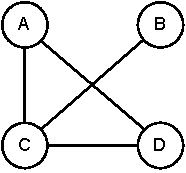
\includegraphics[width=4cm]{mygraph.pdf}
    \end{center}
    
    \caption{An example of a visualisation of a graph.  Figures should always have a caption so that the reader understands its purpose.}\label{fig:mygraph}
\end{figure}

\section{Python code}
Although you won't have significant amounts of Python code in your project report, you will likely want to mention variable names, module names, file names, and the like.  These are usually typset using a fixed-width or typewriter font, like so: \verb+graphs.distanceClasses()+.

\section{Structure}
For your report the main structure will be to divide the report into one section for each task.  Beyond that, you should make appropriate use of paragraphs to organise sentences around ideas.

\section{Citing your sources}
It is considered good academic practice to clearly indicate when you are using content or ideas from others and to cite your sources.  If you copy directly from someone else you should either use quotation marks or, for longer quotations, indent.  For example, ``a \emph{graph} is an irreflexive, symmetric relation.'' (\cite{cab203lecture7}, slide 5).  A longer example from the QUT Cite Write page is: 
\begin{quote}
    You should not use material from previous assignments unless you have permission from your unit coordinator. Some assessments are split into two parts and you need to reuse or refer to the first part in the second. If you think this is the case, check your assignment information. If you are still not sure ask the Unit Coordinator.~\cite{citewrite}
\end{quote}
Even if you don't copy directly, you should also cite sources of specific information that is not common knowledge.  Properly citing your sources avoids plagiarism~\cite{citewrite}.  It is also common to cite a reference for the reader when a new topic is introduced so that they can learn more about that topic if they are new to it.  For example, you might want to cite one of the textbooks as a reference for graphs (for more information about graphs, see~\cite{voloshintextbook}).

You can use any common citation and bibiography styles you like, as long as you are consistent.  QUT's Cite Write page \cite{citewrite} has information about some common styles.

\section{Software}
Typesetting mathematics is a bit of a specialist task, but there is a lot of software that can help.  Almost all of the unit content is typeset using \LaTeX, and that is the easiest way to get consistently good results.  It does require some learning, but for this unit you won't need to get too deep into it.  Unless you are strongly against learning a new language you should at least have a look.

Some software that you may find useful:
\begin{itemize}
    \item Overleaf online \LaTeX editor: \url{https://www.overleaf.com}
    \item TeX Live \LaTeX distribution: \url{https://tug.org/texlive/}
    \item TeXstudio \LaTeX editor: \url{https://www.texstudio.org}
    \item LibreOffice has an equation editor: \url{https://www.libreoffice.org}
    \item diagrams.net for figures: \url{https://diagrams.net}
    \item MS Word has an equation editor 
\end{itemize}

\begin{thebibliography}{9}
    \bibitem{diagramsnet}
        \emph{diagrams.net},
        \url{https://www.diagrams.net/}
        Accessed 12/04/2023.
    \bibitem{cab203lecture7}
        Matthew McKague,
        \emph{CAB203 Lecture 7}.
        \url{https://canvas.qut.edu.au/courses/1979/files/1701728/download?download_frd=1}
        QUT, 2023.
    \bibitem{citewrite}
        QUT,
        \emph{QUT cite tool}.
        \url{https://www.citewrite.qut.edu.au/cite/qutcite.html}
        Accessed 12/04/2023.
    \bibitem{cab203graphs.py}
        Matthew McKague,
        \emph{graphs.py}.
        \url{https://canvas.qut.edu.au/courses/1979/files/1755763/download?download_frd=1}
        QUT, 2023.
    \bibitem{voloshintextbook}
        Vitaly Voloshin,
        \emph{Introduction to graph theory}.
        New York: Nova Science Publishers, 2009.
    \bibitem{pacetextbook}
        Gordon Pace,
        \emph{Mathematics of discrete structures for computer science},
        1st ed. Berlion: Springer, 2012.
\end{thebibliography}
\end{document}